\documentclass[conference]{IEEEtran}
\IEEEoverridecommandlockouts

\usepackage{cite}
\usepackage{amsmath}
\usepackage{array}
\usepackage{booktabs}
\usepackage{graphicx}
\usepackage{xcolor}
\usepackage{listings}
\usepackage{tikz}
\usepackage{pgfplots}
\usepackage{pgfplotstable}
\usepackage[hidelinks]{hyperref}

\pgfplotsset{compat=1.18}

\lstset{
  basicstyle=\ttfamily\footnotesize,
  breaklines=true,
  frame=single,
  columns=fullflexible,
  backgroundcolor=\color{gray!8}
}

\title{Title of Work: Hybrid BB84 Quantum Key Distribution and AES-256-GCM Encryption System}

\author{
\IEEEauthorblockN{Cybersecurity Project}
\IEEEauthorblockA{
Department of Cybersecurity\\
Hybrid Quantum-Classical Cryptography Lab}
}

\begin{document}
\maketitle

\begin{abstract}
\textbf{What:} This paper presents a hybrid encryption system that combines a software simulation of the BB84 quantum key distribution protocol with AES-256-GCM authenticated encryption. The BB84 layer establishes a shared secret bit string between Alice and Bob, while the AES-GCM layer encrypts and authenticates the actual plaintext message.

\textbf{Why:} Classical public-key key exchange methods are threatened by large-scale quantum computation because Shor's algorithm can solve integer factorization and discrete logarithms in polynomial time \cite{shor1997polynomial}. AES remains efficient for bulk encryption, but it still requires a safely distributed symmetric key. BB84 addresses the key-distribution problem by using quantum measurement disturbance to detect eavesdropping \cite{bennett1984bb84}.

\textbf{How:} Alice and Bob are modeled with random bit and basis generation, simulated qubit encoding, random measurement, basis reconciliation, QBER estimation, simplified reconciliation, and privacy amplification. If QBER exceeds an 11\% threshold, the key exchange aborts. Otherwise, SHAKE-256 compresses the reconciled bit string into a 256-bit key, which is then used by AES-256-GCM. The implementation is validated through unit tests, a three-scenario demo, and graph-based QBER analysis.
\end{abstract}

\begin{IEEEkeywords}
BB84, quantum key distribution, QBER, AES-256-GCM, privacy amplification, cybersecurity.
\end{IEEEkeywords}

\section{Problem Statement}
Secure communication requires both secret-key establishment and protected data transmission. In conventional systems, public-key cryptography is often used to exchange or wrap a symmetric key, and a symmetric cipher is then used to encrypt bulk data. This design is efficient, but its security depends on computational hardness assumptions. Shor's quantum algorithm demonstrates that the assumptions behind RSA, finite-field Diffie--Hellman, and elliptic-curve Diffie--Hellman are vulnerable to a sufficiently capable quantum computer \cite{shor1997polynomial}.

Quantum key distribution (QKD) changes the key-establishment model. In BB84, Alice sends randomly chosen bits encoded in randomly chosen conjugate bases, and Bob measures each received state using his own random bases. After transmission, they publicly compare only their basis choices and keep the positions where the bases match. If an eavesdropper Eve intercepts and measures the quantum states, her measurement disturbs some states and introduces detectable errors in the sifted key \cite{bennett1984bb84}.

However, BB84 alone does not encrypt large user messages. It produces shared key material. That key material must be processed through QBER estimation, reconciliation, and privacy amplification before it can safely drive a classical cipher. The problem addressed in this project is therefore to build a complete educational pipeline that demonstrates how a BB84-derived key can be used with AES-256-GCM for practical authenticated encryption.

The project also addresses a learning gap in cybersecurity laboratories. Students often study symmetric encryption, public-key key exchange, and post-quantum threats as separate topics. This separation can hide an important engineering reality: a secure communication system is not a single algorithm, but a chain of assumptions and transformations. A QKD protocol must still handle noisy measurements, information leaked during public discussion, key-length requirements, and safe use of the final key. A symmetric cipher must still be paired with a sound key-establishment process. The proposed project therefore treats the hybrid design as a system problem rather than a standalone algorithm exercise.

The specific threat model is an intercept-resend adversary. Eve does not break AES directly and does not exploit implementation side channels. Instead, she tries to learn the BB84 key by measuring qubits in transit. This is the classic attack used to explain BB84's disturbance principle. When Eve chooses the wrong basis, she changes the state that Bob receives. Alice and Bob cannot identify every disturbed qubit individually, but they can estimate the error rate by sacrificing a sample of their sifted key. If the sample error rate is too high, they reject the session before any AES encryption occurs.

\section{Objective 1: Implement a BB84 Key Distribution Simulator}
The first objective is to implement a clean BB84 simulation with Alice, Bob, and a quantum channel abstraction. Alice must generate random bits and random bases, encode them as simulated qubit states, and announce bases during reconciliation. Bob must independently choose random bases, measure the received states, and keep only matching-basis positions. On a clean channel, the sifted keys should match exactly and the sifted-key ratio should remain close to 50\%, because Alice and Bob choose from two bases independently.

This objective is validated by checking the shape and domain of Alice's generated arrays, verifying that encoded qubit states remain in the set $\{0,1,2,3\}$, and confirming that Alice and Bob obtain identical sifted keys on a clean channel. The 50\% sifting result is not an implementation artifact; it follows from the probability that two independent random basis choices are equal.

\section{Objective 2: Detect Eavesdropping and Distill a Usable Key}
The second objective is to model Eve and convert raw BB84 output into usable symmetric key material. Eve is implemented as an intercept-resend attacker who measures a configurable fraction of qubits in random bases and then re-sends her measured states. This behavior should raise the quantum bit error rate (QBER). The implementation estimates QBER from a sacrificed sample, aborts above the threshold, reconciles remaining key disagreements, and applies privacy amplification. Privacy amplification is essential because reconciliation and any Eve observations may leak partial information about the raw key \cite{bennett1995privacy}.

This objective is validated through a QBER sweep. Instead of only testing whether Eve is detected at 100\% interception, the system records the measured QBER for intercept rates from 0\% to 100\%. This gives a more useful analysis because it demonstrates the gradual relationship between Eve's information-gathering attempt and Alice/Bob's observed disturbance.

\section{Objective 3: Integrate AES-256-GCM Encryption}
The third objective is to connect the distilled 256-bit BB84 key to AES-256-GCM. AES is standardized by NIST as a symmetric block cipher \cite{nist197}, and GCM provides authenticated encryption with integrity checking \cite{nist38d}. The implementation must support successful encryption/decryption with the correct key and must reject wrong keys or tampered ciphertext through the GCM authentication tag.

This objective is validated with roundtrip encryption tests, wrong-key tests, and tampered-ciphertext tests. The final hybrid demonstration is considered successful only if BB84 produces an acceptable key, AES-GCM encrypts the plaintext, and decryption recovers the exact original message.

\section{Scope of Work}
This project is scoped as a third-year cybersecurity lab implementation. It uses a software simulation of BB84 rather than real optical hardware. Qubits are represented as state indices from 0 to 3, where each index combines one basis value and one bit value. The channel can run cleanly or with Eve present. The AES layer uses the Python \texttt{cryptography} library rather than a custom AES implementation.

The scope includes BB84 simulation, intercept-resend eavesdropping, QBER estimation, simplified reconciliation, SHAKE-256 privacy amplification, AES-256-GCM encryption, unit tests, demo execution, and result analysis. The scope excludes physical photon transmission, detector modeling, authenticated public-channel infrastructure, full finite-key proofs, and production-grade QKD reconciliation.

\begin{table}[htbp]
\caption{Scope Boundary of the Project}
\centering
\begin{tabular}{p{0.43\columnwidth}p{0.43\columnwidth}}
\toprule
\textbf{Included} & \textbf{Excluded} \\
\midrule
Software BB84 simulation & Physical photon hardware \\
Intercept-resend Eve model & Side-channel attack modeling \\
QBER threshold decision & Full finite-key security proof \\
Simplified reconciliation & Production Cascade/LDPC protocol \\
SHAKE-256 key compression & Hardware random-number source audit \\
AES-256-GCM encryption & Custom AES primitive design \\
\bottomrule
\end{tabular}
\label{tab:scope}
\end{table}

\section{Existing Approaches and Gaps/Improvement Areas}
\subsection{Classical Public-Key Key Exchange}
RSA, Diffie--Hellman, and elliptic-curve Diffie--Hellman are widely deployed because they work over normal digital networks. Their gap is that they depend on mathematical assumptions vulnerable to quantum algorithms \cite{shor1997polynomial}. The improvement area is quantum-safe key establishment or post-quantum migration.

In a conventional TLS-style system, the application may use AES for the data channel, but the AES key is established through a public-key mechanism. If that public-key mechanism is later broken, recorded traffic may become vulnerable depending on the protocol and whether forward secrecy was used. This creates the ``harvest now, decrypt later'' concern for long-lived confidential data. BB84 responds to this concern by making the key exchange depend on measurement disturbance rather than factorization or discrete logarithm hardness.

\subsection{AES-Only Symmetric Encryption}
AES is fast, standardized, and appropriate for bulk encryption \cite{nist197}. AES-GCM also detects tampering and wrong-key use \cite{nist38d}. The gap is that AES does not solve key distribution. A strong AES implementation still fails if its secret key is shared insecurely.

An AES-only laboratory project is useful for learning confidentiality and integrity, but it can accidentally make the key appear as a given input. In real systems, key generation and distribution are often the most fragile parts of the design. This project improves on AES-only demonstrations by showing where the AES key comes from and why that source matters.

\subsection{BB84-Only Key Distribution}
BB84 provides a way to generate shared secret bits and detect measurement disturbance \cite{bennett1984bb84}. The gap is that BB84 is not a bulk encryption algorithm. Raw BB84 output requires sifting, error estimation, reconciliation, and privacy amplification before it is suitable as a symmetric key \cite{bennett1995privacy,scarani2009security}.

A BB84-only simulation may stop when Alice and Bob obtain a sifted key. That is incomplete from a security-engineering perspective. The sifted key may contain errors and may be partially known to Eve. It may also have a variable length. A real encryption system needs a fixed-size key with a well-defined security interpretation. This project therefore connects BB84 output to privacy amplification and then to AES-256-GCM.

\subsection{Post-Quantum Cryptography}
Post-quantum cryptography such as NIST ML-KEM is designed for deployment over existing classical networks \cite{nist203}. Its gap, compared with QKD, is that it remains computational cryptography. QKD and PQC solve related problems through different assumptions; practical systems may compare or combine both approaches.

\begin{table*}[htbp]
\caption{Approaches, Gaps, and Improvement Areas}
\centering
\begin{tabular}{p{0.18\textwidth}p{0.25\textwidth}p{0.25\textwidth}p{0.22\textwidth}}
\toprule
\textbf{Approach} & \textbf{Strength} & \textbf{Gap} & \textbf{Improvement Area} \\
\midrule
Classical public-key exchange & Mature, scalable, no special channel & Vulnerable to future quantum attacks for RSA/DH/ECDH & Replace or supplement with QKD/PQC \\
AES-only encryption & Fast, standardized, practical for data & Does not distribute keys & Pair with secure key establishment \\
BB84-only simulation & Demonstrates quantum disturbance & Does not encrypt bulk data and lacks full post-processing & Add reconciliation, privacy amplification, and AES \\
PQC key encapsulation & Deployable on existing networks & Computational assumptions remain & Compare with or combine with QKD \\
\bottomrule
\end{tabular}
\label{tab:gaps}
\end{table*}

\section{Novelty/Innovativeness in Project}
The novelty of this project lies in the end-to-end educational integration. Many BB84 examples stop at sifted key generation, while many AES demonstrations assume that a key already exists. This project joins both sides: BB84 produces a key candidate, key-distillation logic makes it suitable for cryptographic use, and AES-GCM encrypts the actual message.

The project is also analysis-driven. It does not merely state that Eve is detectable; it plots how QBER changes as Eve's intercept rate increases. It also shows that the sifted-key ratio remains stable near 50\%, while the abort rate rises as QBER crosses the security threshold. This makes the statistical behavior of BB84 visible and measurable.

Another innovative aspect is that the project treats failed sessions as correct behavior. In ordinary encryption demos, success often means producing ciphertext. In this hybrid system, refusing to encrypt is also a security success when QBER indicates a compromised channel. This is an important lesson: secure systems should fail closed when their assumptions are violated.

\section{Proposed Method}
The proposed method has two connected layers: a BB84 key-establishment layer and an AES-GCM encryption layer. Fig.~\ref{fig:method} summarizes the complete flow.

\begin{figure}[htbp]
\centering
\resizebox{\columnwidth}{!}{
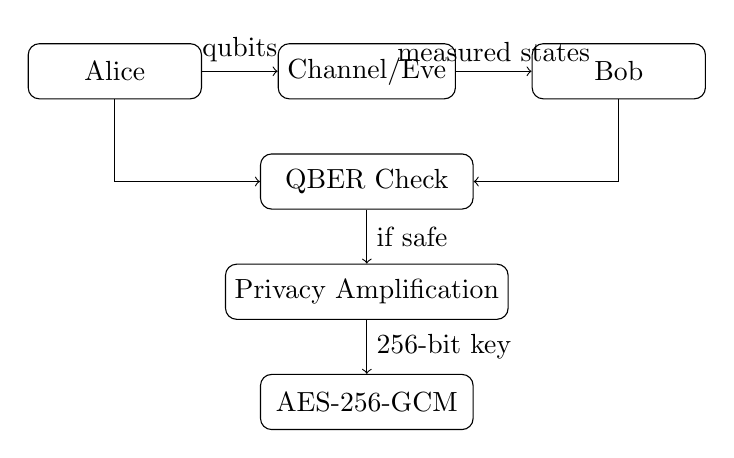
\begin{tikzpicture}
\node[draw, rounded corners, minimum width=2.2cm, minimum height=0.7cm] (a) at (0,0) {Alice};
\node[draw, rounded corners, minimum width=2.2cm, minimum height=0.7cm] (c) at (3.2,0) {Channel/Eve};
\node[draw, rounded corners, minimum width=2.2cm, minimum height=0.7cm] (b) at (6.4,0) {Bob};
\node[draw, rounded corners, minimum width=2.7cm, minimum height=0.7cm] (q) at (3.2,-1.4) {QBER Check};
\node[draw, rounded corners, minimum width=2.7cm, minimum height=0.7cm] (p) at (3.2,-2.8) {Privacy Amplification};
\node[draw, rounded corners, minimum width=2.7cm, minimum height=0.7cm] (aes) at (3.2,-4.2) {AES-256-GCM};
\draw[->] (a) -- node[above]{qubits} (c);
\draw[->] (c) -- node[above]{measured states} (b);
\draw[->] (b) |- (q);
\draw[->] (a) |- (q);
\draw[->] (q) -- node[right]{if safe} (p);
\draw[->] (p) -- node[right]{256-bit key} (aes);
\end{tikzpicture}}
\caption{Proposed hybrid BB84 and AES-256-GCM workflow.}
\label{fig:method}
\end{figure}

\subsection{BB84 Layer}
Alice generates random bits and bases. The implementation maps each simulated qubit state using
\begin{equation}
\text{state} = 2 \times \text{basis} + \text{bit}.
\end{equation}
Bob chooses random bases and measures the received states. If Bob's basis matches Alice's basis, the bit is deterministic. If the bases differ, the measured bit is random and later discarded.

The expected sifted-key length is approximately $n/2$ for $n$ transmitted qubits:
\begin{equation}
E[|K_s|] = n \cdot P(b_A=b_B)=n \cdot \frac{1}{2}.
\end{equation}
This expectation is visible in the experimental sweep, where the sifted-key ratio remains near 0.5 even when Eve is present. Eve changes the correctness of some retained bits, not the probability that Alice and Bob choose the same basis.

\subsection{Eavesdropper and QBER Decision}
Eve measures intercepted qubits in random bases. With full intercept-resend, she chooses the wrong basis about half the time. When Alice and Bob later keep matching-basis positions, those disturbed cases create an expected QBER near 25\%. The project aborts when estimated QBER exceeds 11\%.

The simplified expected relationship between intercept rate $r$ and QBER is
\begin{equation}
QBER \approx r \times \frac{1}{2} \times \frac{1}{2} = \frac{r}{4}.
\end{equation}
The first factor is Eve's interception probability, the second is the probability that Eve selects the wrong basis, and the third is the probability that Bob receives the wrong bit after that disturbance. This simple model explains why full interception tends toward 25\% QBER and why partial interception can be harder to detect in a small sample.

\subsection{Key Distillation and AES Layer}
After QBER sampling, the remaining bits are reconciled. Privacy amplification then uses SHAKE-256 as a hash extractor to produce a 256-bit AES key. AES-GCM encrypts the plaintext with a 96-bit nonce and additional authenticated data. The authentication tag protects against ciphertext tampering, wrong-key decryption, and AAD mismatch.

The project intentionally separates key establishment from message encryption. The BB84 layer decides whether key material is safe enough to use. The AES layer does not know whether Eve was present; it only receives a 32-byte key. This separation mirrors real cryptographic engineering, where protocol layers should have clear responsibilities.

\section{Implementation and Result}
\subsection{Implementation Summary}
The implementation is organized as Python modules. \texttt{alice.py}, \texttt{bob.py}, and \texttt{channel.py} implement the BB84 actors and channel. \texttt{reconciliation.py} estimates QBER and corrects Bob's key. \texttt{privacy\_amplification.py} derives the final 256-bit key. \texttt{aes\_cipher.py} wraps AES-256-GCM. \texttt{bb84\_pipeline.py} orchestrates key distribution, while \texttt{hybrid\_encrypt.py} combines key generation with message encryption.

\begin{table*}[htbp]
\caption{Implementation Module Mapping}
\centering
\begin{tabular}{p{0.20\textwidth}p{0.34\textwidth}p{0.34\textwidth}}
\toprule
\textbf{Module} & \textbf{Responsibility} & \textbf{Relation to BB84 + AES} \\
\midrule
\texttt{alice.py} & Generates Alice's random bits and bases; encodes simulated qubits & Starts BB84 key establishment \\
\texttt{bob.py} & Chooses measurement bases and measures received states & Produces Bob's raw measured key \\
\texttt{channel.py} & Passes qubits cleanly or applies Eve intercept-resend & Models quantum-channel disturbance \\
\texttt{reconciliation.py} & Estimates QBER and corrects Bob's remaining bits & Decides whether key material is safe to continue \\
\texttt{privacy\_amplification.py} & Packs bits and derives a fixed 256-bit key & Converts reconciled bits into AES key material \\
\texttt{aes\_cipher.py} & Encrypts/decrypts using AES-256-GCM & Provides authenticated bulk encryption \\
\texttt{bb84\_pipeline.py} & Runs the full BB84 sequence & Produces final key or aborts \\
\texttt{hybrid\_encrypt.py} & Bridges BB84 output to AES-GCM & Implements the full hybrid system \\
\bottomrule
\end{tabular}
\label{tab:modules}
\end{table*}

\begin{lstlisting}
1. Alice generates bits and BB84 bases.
2. Alice sends simulated qubit states.
3. Eve optionally intercepts and re-sends states.
4. Bob measures with random bases.
5. Alice and Bob keep matching-basis positions.
6. A sample estimates QBER.
7. High QBER aborts the session.
8. Safe keys are reconciled and compressed.
9. AES-256-GCM encrypts the message.
\end{lstlisting}

\subsection{Demo Results}
The system was executed with three scenarios. A clean channel encrypted and decrypted successfully. Full interception produced QBER near the theoretical 25\% level and aborted. Partial interception produced lower QBER and may remain below the abort threshold.

\begin{table}[htbp]
\caption{Representative Demo Result}
\centering
\begin{tabular}{lccc}
\toprule
\textbf{Scenario} & \textbf{QBER} & \textbf{Action} & \textbf{Status} \\
\midrule
Clean channel & 0.00\% & Encrypt & Pass \\
Eve 100\% & 25.49\% & Abort & Pass \\
Eve 30\% & 6.47\% & Continue & Observed \\
\bottomrule
\end{tabular}
\label{tab:demo}
\end{table}

\subsection{Graph Analysis: QBER vs Intercept Rate}
Fig.~\ref{fig:qber} shows that QBER increases as Eve intercepts more qubits. The dashed line marks the 11\% abort threshold. In the recorded sweep, the average QBER crosses the threshold around 50\% interception.

The graph is also useful because it separates two ideas that are often confused. Eve's intercept rate is not the same as QBER. If Eve intercepts every qubit, she still chooses the correct basis about half the time. Even when she chooses the wrong basis, the final bit is wrong only probabilistically. Therefore, the observed QBER is lower than the intercept rate. This is why the slope of the measured curve is close to one quarter rather than one.

\begin{figure}[htbp]
\centering
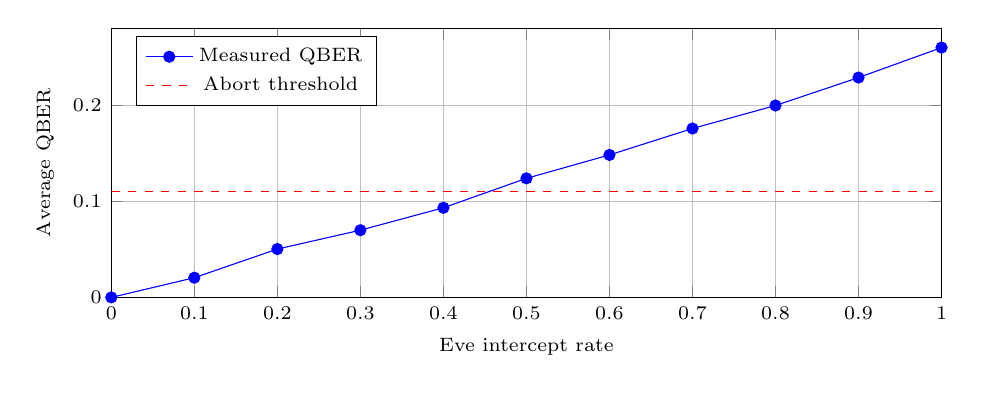
\begin{tikzpicture}
\begin{axis}[
  width=\columnwidth,
  height=5cm,
  xlabel={Eve intercept rate},
  ylabel={Average QBER},
  xmin=0, xmax=1,
  ymin=0, ymax=0.28,
  grid=both,
  legend pos=north west,
  tick label style={font=\scriptsize},
  label style={font=\scriptsize},
  legend style={font=\scriptsize}
]
\addplot[color=blue, mark=*] coordinates {
  (0.0,0.000000) (0.1,0.020469) (0.2,0.050286)
  (0.3,0.069905) (0.4,0.093230) (0.5,0.123827)
  (0.6,0.148194) (0.7,0.175676) (0.8,0.199614)
  (0.9,0.228656) (1.0,0.259846)
};
\addlegendentry{Measured QBER}
\addplot[color=red, dashed, domain=0:1] {0.11};
\addlegendentry{Abort threshold}
\end{axis}
\end{tikzpicture}
\caption{QBER increases with Eve's intercept rate.}
\label{fig:qber}
\end{figure}

\subsection{Graph Analysis: Sifted-Key Ratio}
Fig.~\ref{fig:sifted} shows that the sifted-key ratio remains close to 0.5 across all intercept rates. This is expected because sifting depends mainly on whether Alice and Bob chose the same basis, not on whether Eve was present.

This graph confirms that the simulator is not accidentally discarding more bits when Eve is present. Eve changes the reliability of retained bits, while basis reconciliation controls the retained-bit count. A stable sifted ratio makes the QBER trend easier to interpret because changes in QBER are not caused by major changes in sample size.

\begin{figure}[htbp]
\centering
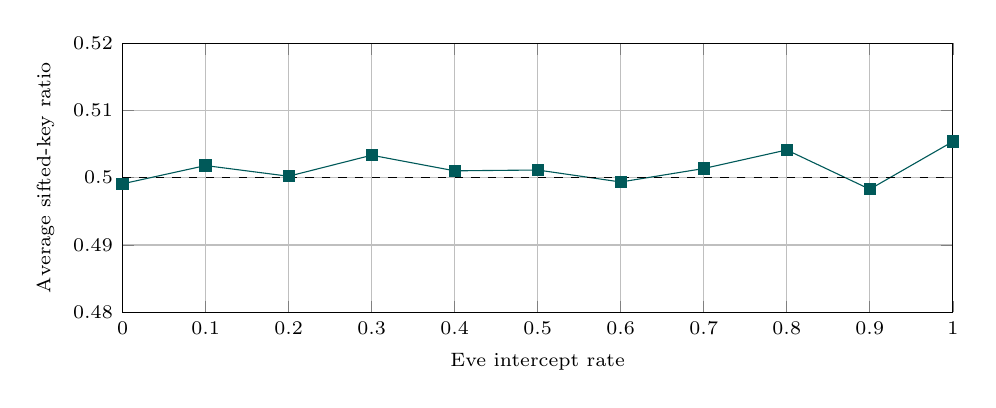
\begin{tikzpicture}
\begin{axis}[
  width=\columnwidth,
  height=5cm,
  xlabel={Eve intercept rate},
  ylabel={Average sifted-key ratio},
  xmin=0, xmax=1,
  ymin=0.48, ymax=0.52,
  grid=both,
  tick label style={font=\scriptsize},
  label style={font=\scriptsize}
]
\addplot[color=teal!70!black, mark=square*] coordinates {
  (0.0,0.499097) (0.1,0.501807) (0.2,0.500220)
  (0.3,0.503345) (0.4,0.501025) (0.5,0.501147)
  (0.6,0.499365) (0.7,0.501367) (0.8,0.504126)
  (0.9,0.498291) (1.0,0.505371)
};
\addplot[color=black, dashed, domain=0:1] {0.5};
\end{axis}
\end{tikzpicture}
\caption{The sifted-key ratio remains near the theoretical 50\% value.}
\label{fig:sifted}
\end{figure}

\subsection{Graph Analysis: Abort Behavior}
Fig.~\ref{fig:abort} plots aborted trials out of five runs per intercept rate. The result shows that abort probability rises sharply once QBER crosses the threshold. The 40\% case produced only one abort because measured QBER was still often below 11\%, while 50\% and above were mostly or fully rejected.

The abort graph highlights the statistical nature of BB84 detection. A single partial-interception session may pass if the sampled bits do not produce QBER above the threshold. This does not mean Eve is harmless. It means that security decisions depend on sample size, threshold selection, channel noise, and the amount of privacy amplification. A production QKD system would use finite-key bounds rather than the simple threshold used in this lab.

\begin{figure}[htbp]
\centering
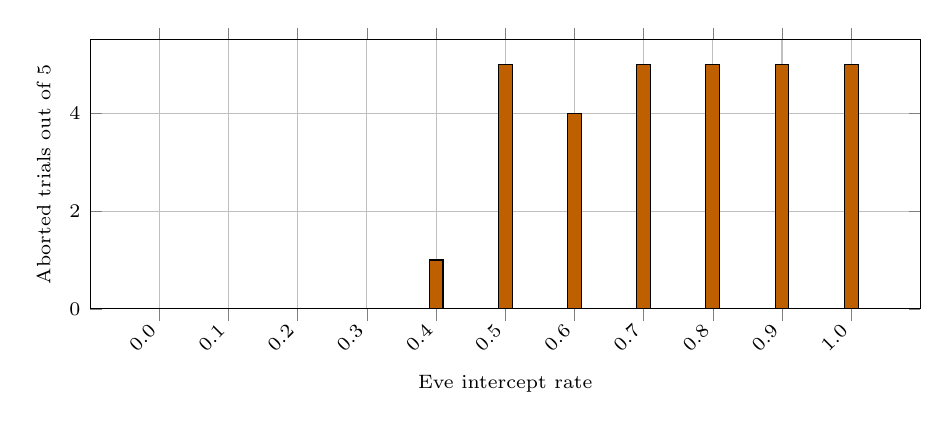
\begin{tikzpicture}
\begin{axis}[
  ybar,
  width=\columnwidth,
  height=5cm,
  xlabel={Eve intercept rate},
  ylabel={Aborted trials out of 5},
  ymin=0, ymax=5.5,
  symbolic x coords={0.0,0.1,0.2,0.3,0.4,0.5,0.6,0.7,0.8,0.9,1.0},
  xtick=data,
  x tick label style={rotate=45, anchor=east, font=\scriptsize},
  tick label style={font=\scriptsize},
  label style={font=\scriptsize},
  grid=major,
  bar width=5pt
]
\addplot[fill=orange!75!black] coordinates {
  (0.0,0) (0.1,0) (0.2,0) (0.3,0) (0.4,1)
  (0.5,5) (0.6,4) (0.7,5) (0.8,5) (0.9,5) (1.0,5)
};
\end{axis}
\end{tikzpicture}
\caption{Session aborts increase after QBER crosses the security threshold.}
\label{fig:abort}
\end{figure}

\subsection{Tabulated Sweep Result}
Table~\ref{tab:sweep} lists the measured sweep values. The clean-channel QBER is 0, while full interception approaches the theoretical 25\% value.

\begin{table*}[htbp]
\caption{QBER Sweep Result Across Eve Intercept Rates}
\centering
\begin{tabular}{cccccccccccc}
\toprule
\textbf{Rate} & 0.0 & 0.1 & 0.2 & 0.3 & 0.4 & 0.5 & 0.6 & 0.7 & 0.8 & 0.9 & 1.0 \\
\midrule
\textbf{Avg. QBER} & .000 & .020 & .050 & .070 & .093 & .124 & .148 & .176 & .200 & .229 & .260 \\
\textbf{Sifted Ratio} & .499 & .502 & .500 & .503 & .501 & .501 & .499 & .501 & .504 & .498 & .505 \\
\textbf{Aborts/5} & 0 & 0 & 0 & 0 & 1 & 5 & 4 & 5 & 5 & 5 & 5 \\
\bottomrule
\end{tabular}
\label{tab:sweep}
\end{table*}

\subsection{Validation}
The test suite collected 17 tests and all passed. The tests validate Alice's data generation, clean-channel key agreement, approximate 50\% sifting, Eve-induced QBER, pipeline abort behavior, reconciliation, privacy-amplification length, AES roundtrip encryption, wrong-key rejection, ciphertext tamper detection, and full hybrid encrypt/decrypt.

\begin{table}[htbp]
\caption{Security Property Validation}
\centering
\begin{tabular}{p{0.40\columnwidth}p{0.45\columnwidth}}
\toprule
\textbf{Property} & \textbf{Validation Method} \\
\midrule
Clean BB84 agreement & Alice/Bob sifted-key equality test \\
Eve disturbance & QBER above threshold under full intercept \\
Key length correctness & 32-byte privacy-amplified output \\
AES confidentiality path & Encrypt/decrypt roundtrip test \\
Wrong-key rejection & AES-GCM InvalidTag exception \\
Tamper detection & Modified ciphertext fails decryption \\
\bottomrule
\end{tabular}
\label{tab:validation}
\end{table}

The implementation uses AES-GCM from a standard cryptographic library rather than implementing AES manually. This is important because custom cipher implementations can introduce timing bugs, incorrect padding behavior, nonce misuse, or authentication mistakes. The educational focus is on hybrid protocol composition, so a vetted AES-GCM primitive is the safer engineering choice.

\section{Conclusion}
The project successfully implements a hybrid BB84 + AES encryption system in IEEE-style research form. BB84 is used to establish the symmetric key, while AES-256-GCM is used for efficient authenticated encryption of the message. The results show that a clean channel generates matching key material and supports AES encryption, while a full intercept-resend Eve raises QBER near 25\% and causes the session to abort.

The graphs support the expected theory: QBER increases with Eve's intercept rate, the sifted-key ratio remains close to 50\%, and aborts become frequent after the measured QBER exceeds the threshold. Therefore, the implementation meets the educational goal of connecting quantum key distribution concepts with classical symmetric encryption in a measurable cybersecurity project.

\section{Future Work}
Future work can improve both realism and security. The simplified reconciliation function can be replaced with a full Cascade or LDPC-based reconciliation protocol. The public classical channel should be authenticated to prevent man-in-the-middle attacks. Finite-key analysis can be added to account for statistical uncertainty in QBER sampling.

The channel model can also be extended with photon loss, detector dark counts, optical misalignment, and background noise. A future version may compare BB84 with post-quantum key encapsulation such as ML-KEM \cite{nist203}, or build a hybrid demonstration where PQC authenticates the classical channel and BB84 supplies the session key. A graphical dashboard could further improve learning by visualizing basis choices, discarded bits, QBER, abort decisions, and AES-GCM ciphertext output.

\begin{thebibliography}{00}
\bibitem{bennett1984bb84}
C. H. Bennett and G. Brassard, ``Quantum cryptography: Public key distribution and coin tossing,'' in \emph{Proc. IEEE Int. Conf. Computers, Systems and Signal Processing}, Bangalore, India, pp. 175--179, 1984.

\bibitem{bennett1992experimental}
C. H. Bennett, F. Bessette, G. Brassard, L. Salvail, and J. Smolin, ``Experimental quantum cryptography,'' \emph{Journal of Cryptology}, vol. 5, no. 1, pp. 3--28, 1992.

\bibitem{bennett1995privacy}
C. H. Bennett, G. Brassard, C. Crepeau, and U. M. Maurer, ``Generalized privacy amplification,'' \emph{IEEE Transactions on Information Theory}, vol. 41, no. 6, pp. 1915--1923, 1995.

\bibitem{shor1997polynomial}
P. W. Shor, ``Polynomial-time algorithms for prime factorization and discrete logarithms on a quantum computer,'' \emph{SIAM Journal on Computing}, vol. 26, no. 5, pp. 1484--1509, 1997.

\bibitem{scarani2009security}
V. Scarani, H. Bechmann-Pasquinucci, N. J. Cerf, M. Dusek, N. Lutkenhaus, and M. Peev, ``The security of practical quantum key distribution,'' \emph{Reviews of Modern Physics}, vol. 81, no. 3, pp. 1301--1350, 2009.

\bibitem{nist197}
National Institute of Standards and Technology, \emph{Advanced Encryption Standard (AES)}, FIPS PUB 197, updated 2023.

\bibitem{nist38d}
M. J. Dworkin, \emph{Recommendation for Block Cipher Modes of Operation: Galois/Counter Mode (GCM) and GMAC}, NIST Special Publication 800-38D, 2007.

\bibitem{nist203}
National Institute of Standards and Technology, \emph{Module-Lattice-Based Key-Encapsulation Mechanism Standard}, FIPS PUB 203, 2024.
\end{thebibliography}

\end{document}
